在本书的这一部分, 我们在强化学习最简单的形式下——状态与动作空间足够小使得近似的值函数可以以数组或\emph{表}<table>来表示——阐述几乎所有强化学习算法的核心概念. 在这种情况下, 这些方法常常可以获得确切的解, 即可以获得确切的最优值函数与最优策略. 这和本书的下一部分叙述的近似方法恰恰相反, 后者只能获得近似解, 但作为回报可以高效地应用于规模大得多的问题上.

本书这一部分的第一章阐述了只有单个状态的强化学习问题特例, 即所谓的赌博机问题. 第二章阐述了在本书的余下部分使用的、一般强化学习问题的形式化——有限马尔科夫决策过程<finite Markov decision process, finite MDP>, 也阐述了形式化中包括了贝尔曼方程<Bellman equation>与值函数的主要概念.

接下来的三章阐述了三类解决有限马尔科夫决策过程的基本方法: 动态规划<dynamic programming, DP>, 蒙特卡洛<Monte Carlo, MC>方法, 以及时序差分<temporal difference, TD>方法. 每一类方法都有其优点与缺点. 动态规划方法在数学上被研究得很好, 但需要完整、正确的环境模型. 蒙特卡洛方法不需要模型且从概念上说较为简单, 但不适合于逐步的增量计算. 最后, 时序差分方法不需要模型且完全是增量式的, 但分析起来更为复杂. 这些方法在效率与收敛速度这些方面也存在着差异.

余下的两章阐述了怎么将这三类方法结合起来以利用各自的优点. 在其中一章我们阐述怎样通过多步自举方法<multi-step bootstrapping method>来将蒙特卡洛方法与时序差分方法的长处结合起来. 在本部分的最后一章, 我们将展示怎样将时序差分学习方法, 与模型学习以及计划方法(例如动态规划)结合起来, 作为完整、统一的表格式强化学习问题的解决方案.

\chapter{多摇臂赌博机}\label{chap:2}

将强化学习同其他类型的学习区分开来的最重要的特征就是: 强化学习使用训练信息来\emph{评估}所采取的动作, 而非使用正确的动作来\emph{指导}动作的选择. 正是这一点提出了对积极探索的要求. 单纯的评估性反馈只能说明所采取的动作的好坏, 但无法说明其是否为最好或最坏的动作. 单纯的指示性反馈, 恰恰相反, 指示出应该做的正确动作, 且独立于实际采取的动作. 这一类的反馈是包含了大量模式分类、人工神经网络、系统辨别的监督学习的基础. 在各自最典型的情况下, 这两类反馈是大不相同的: 评估性反馈完全依赖于所采取的动作, 而指示性反馈独立于所采取的动作.

在本章中我们在简化的设定下——仅需要在单个状态下学得如何采取动作——来探讨强化学习评估的方面. 多数涉及到评估性反馈的先前工作正是在这个\emph{非关联性}<nonassociative>设定下完成的, 因为这个设定避免了完整强化学习问题的复杂性. 学习这种情形使我们能清晰地看到评估性反馈怎样地区别于指示性反馈, 又怎样地可以同指示性反馈结合起来.

我们探讨的非关联性的评估性反馈问题正是$k$-摇臂赌博机问题<$k$-armed bandit problem>的一种简单形式. 我们利用这个问题来介绍一些基本的强化学习方法, 并在之后的章节中拓展这些方法以应用于完整的强化学习问题上. 在本章的末尾, 我们探讨赌博机问题变成关联性——即需要在多个状态下采取动作——时会发生什么, 来向完整的强化学习问题更进一步.

% ----------------------------------- sec2.1 ---------------------------------------------
\section{\texorpdfstring{$k$-摇臂赌博机问题}{k-摇臂赌博机问题}}\label{sec:2.1}

考虑如下的学习问题. 你需要重复地对$k$个不同的选项或动作做出选择. 在每一次选择后你会获得一个实数型的奖赏, 该奖赏是从固定的概率分布中采样获得的, 且该概率分布取决于你所选择的动作. 你的目标在一定的时期内, 如1000个动作选择或\emph{时步}<time step>内, 最大化期望的奖赏和.

这是$k$\emph{-摇臂赌博机问题}<$k$-armed bandit problem>的典型形式, 之所以这么称呼是将其类比于老虎机或``单摇臂赌博机'', 只不过其有$k$个摇臂, 而非1个. 每一次动作选择就像拉下赌博机的摇臂之一, 而奖赏就是中了头奖之后的回报. 在反复的动作选择过程中, 你必须将动作集中到最好的摇臂上来最大化累积奖赏. 另一个类比为, 医生为一批批的重病患者选择实验性的疗法. 每一个动作就是选择一种疗法, 而每一个奖赏就是病人存活或健康与否. 现如今术语``赌博机问题''有时也用于上述问题的泛化, 但本书中我们仅用其指代如上所述的简单形式.

在我们的$k$-摇臂赌博机问题中, $k$个动作中的每一个动作都各自有其期望或平均的奖赏; 让我们将其称为该动作的\emph{值}<value>. 我们将在时步$t$选择的动作记为$A_t$, 对应的奖赏记为$R_t$. 任一动作$a$的值, 记为$q_*(a)$, 为$a$被选择后的期望奖赏:
\begin{equation*}
q_*(a) \doteq \mathbb E [R_t \mid A_t = a].
\end{equation*}
如果你知道了每个动作的值, 那么解决$k$-摇臂赌博机问题就很简单了: 只要一直选择值最高的动作即可. 我们假设你不能确定动作值, 虽然你可能有其估计值. 我们将动作$a$在时步$t$的估计值记为$Q_t(a)$. 我们希望$Q_t(a)$尽可能接近$q_*(a)$.

如果你维持有对动作值的估计, 那么在任何时步一定至少有一个动作有着最高的估计值. 我们将其称为\emph{贪心}<greedy>动作. 当你选择贪心动作之一时, 我们称你在\emph{利用}<exploit>你对动作值的已有知识. 但如果你选择了非贪心动作之一, 那么我们称你在\emph{探索}<explore>, 因为这能帮助你改进对非贪心动作的值的估计. 利用用于最大化单步的期望奖赏, 但探索也许可以在长期内产生更高的奖赏和. 例如, 假设一个贪心动作的值是确定地知道的, 而一些其他的动作以极高的不确定性被估计为和贪心动作差不多好. 这个不确定性为, 这些动作中的至少一个动作, 可能比贪心动作要好, 但你不知道是哪一个. 如果你在选择动作前有许多时步的话, 那么这么做也许会更好: 探索非贪心动作, 来发现其中哪个比贪心动作更好. 在探索过程中, 短期而言奖赏变低了, 但长期而言奖赏会变高, 因为在你发现了更好的动作后, 你可以穿多次地利用\emph{它们}. 因为在单个动作选择中不能既探索又利用, 所有这常常被称为探索与利用之间的``矛盾''.

在任何一个具体的情况下, 是探索还是利用更好取决于对估计值、不确定性、余下步数的具体值的复杂考量. 有许多针对$k$-摇臂赌博机及其关联问题的特定数学形式的、用于平衡探索和利用的精巧方法. 然而, 这些方法中的多数对固定性<stationarity>及先验知识做出了较强的假设, 这些假设对实际应用或我们在接下来的章节中考虑的完整的强化学习问题而言, 要么无法做到, 要么无法证实. 就这些方法而言, 当这些假设不成立时, 其对最优性的保证或对损失的边界的保证, 都无从谈起. 

在本书中我们不考虑以精妙的方式平衡探索和利用; 我们仅以浅显的程度对平衡方法进行探讨. 在本章中我们将呈现数种针对$k$-摇臂赌博机问题的平衡方法, 以及其对只会利用的方法的显著优越性. 需要平衡探索和利用是强化学习特有的特有的挑战; 我们这一版本的$k$-摇臂赌博机问题的简洁性, 使我们能够以一种特别清晰的形式来呈现这一点.

% ----------------------------------- sec2.2 ---------------------------------------------
\section{动作值方法}\label{sec:2.2}

我们以对两种方法的更进一步的审视开始. 这两种方法分别为估计动作值的方法, 以及使用估计值来做出动作选择的决策的方法, 两者合称为\emph{动作值方法}<action-value method>. 我们还记得一个动作的真实值是该动作被选择时的平均奖赏. 一个自然的估计方法就是对接受到的奖赏进行平均:
\begin{equation}\label{eq:2.1}
Q_t(a) = \frac{\text{时步$t$之前采取动作$a$所获得奖赏之和}}{\text{时步$t$之前采取动作$a$的次数}} = \frac{\sum_{i=1}^{t-1}{R_i} \cdot \mathbbm{1}_{A_i = a}}{\sum_{i=1}^{t-1}{\mathbbm{1}_{A_i = a}}}, 
\end{equation}
其中$\mathbbm{1}_{predicate}$表示一随机变量, 当谓词predicate为真时其值为1, 反之为0. 如果分母为0的话, 那么我们可以将$Q_t(a)$设定为一默认值, 比如0. 当分母趋向于无穷大时, 由大数定理可以得知$Q_t(a)$收敛于$q_*(a)$. 我们将此称为估计动作值的\emph{样本平均}方法<sample-average method>, 因为估计值为相关奖赏的样本的均值. 当然这只是估计动作值的一种方法, 也不一定是最好的一种. 但是, 让我们暂且使用这种简单的估计方法, 然后考虑怎样使用估计值来选择动作的问题.

最简单的动作选择规则就是选择有最高估计值的那个动作, 即前一节中定义的贪心动作. 如果有多于一个的贪心动作, 那么以任意一种方式在选择其中一个, 例如随机选择. 我们将这样的\emph{贪心}<greedy>动作选择写作
\begin{equation}\label{eq:2.2}
A_t = \dargmax Q_t(a),
\end{equation}
其中$\targmax_a$表示令后面的表达式最大的那个动作$a$(再次声明, 如果有多个最值时任意选择). 贪心选择总是对已有的知识进行利用来最大化立即的奖赏; 其不会对明显次等的动作进行采样来观察这些动作是否实际上更好. 一个简单的替代方法就是在多数的时间内进行贪心选择; 但是每隔一定时间, 如以一个较小的概率$\varepsilon$, 从所有的动作中以相同的概率进行随机选择, 无论各个动作的估计值为多少. 我们将使用这种近似贪心的动作选择规则的方法称为$\varepsilon$-贪心方法. 这一方法的优点是, 当步数增加到无穷大时, 每个动作都会被采样无穷多次, 因此保证了所有的$Q_t(a)$都收敛到$q_*(a)$. 这也预示着选择最优动作的概率会收敛到大于$1 - \varepsilon$的值, 即几乎确定. 然而这只是一个渐进的保证, 且无法说明该方法的实际效率. 

\begin{exer}
对于$\varepsilon$-贪心动作选择, 在有两个动作并且$\varepsilon = 0.5$的情况下, 贪心动作被选择的概率是多少.
\end{exer}

% ----------------------------------- sec2.3 ---------------------------------------------
\section{10-摇臂测试工具}\label{sec:2.3}

为了大致地评估贪心与$\varepsilon​$-贪心动作值方法的相对效率, 我们使用一个测试问题套件来定量地比较它们. 这是一个由2000个随机生成的$k​$-摇臂赌博机问题组成的集合, 其中$k = 10​$. 对每个赌博机问题而言, 如在\figref{2.1}中所展示的, 各个动作值$q_*(a), \; a= 1, \dots, 10​$, 是从均值为0且方差为1的正态(高斯)分布中采样得到的. 并且, 若一个应用于本问题的学习方法在时步$t​$时选择了动作$A_t​$, 那么实际奖赏$R_t​$是从均值为$q_*(A_t)​$且方差为1的正态分布中采样获得的. 这些分布在\figref{2.1}中用灰色表示. 我们将这个测试任务套件称为\emph{10-摇臂测试工具}. 对于任何学习方法来说, 当将其应用于赌博机问题之一时, 我们可以测量其于1000多个时步中逐步提升的性能与表现. 这构成了一个\emph{行程}<run>. 将此重复2000个独立的行程, 且每个行程使用不同的赌博机问题, 我们获得了对学习算法的平均表现的度量.

\begin{figure}[ht]
\centering
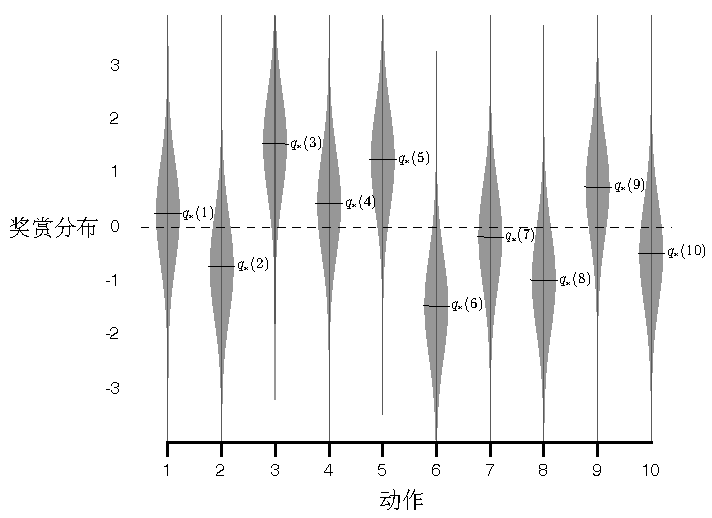
\includegraphics[width=.8\textwidth]{c2/img/figure2-1.pdf}
\caption{一个来自10-摇臂测试工具的赌博机问题示例. 10个动作的真实值$q_*(a)$是从均值为0且方差为1的正态分布中采样得到的, 并且实际奖赏是从均值为$q_*(a)$且方差为1的正态分布中采样得到的.}\label{fig:2.1}
\end{figure}

使用如上所述的10-摇臂测试工具, 对贪心方法以及两个$\varepsilon$-贪心方法($\varepsilon = 0.01$及$\varepsilon = 0.1$)进行对比, 结果如\figref{2.2}所示. 所有方法都使用采样平均方法来估计动作值. 上侧的图展示了随经历增长的期望奖赏. 在最开始, 贪心方法比其他两个方法增长得稍微快一点, 但在一个很低的水平就趋于平稳了. 其只达到了单步奖赏约为1的水准, 而在此测试工具上单步奖赏可能的最大值约为1.55. 贪心方法在长期过程中表现明显相对其他方法更差, 因为其常常陷于对次优动作的选择中. 下侧的图显示贪心方法在大约三分之一的任务中找到了最优动作. 在余下的三分之二任务中, 其对最优动作的初始采样值偏低, 因此最优动作从未被再次选择. $\varepsilon$-贪心方法最终表现得比贪心方法更好, 因为前者持续探索并持续提高发现最优动作的可能. $\varepsilon = 0.1$的方法探索得更多, 所以常常更早地发现最优动作, 但其从不会以超过91\%的概率选择该动作. $\varepsilon = 0.01$的方法提升得更为缓慢, 但最终会在图中的两种测度上比$\varepsilon = 0.1$的方法表现得更好. 也可以随时间逐步减小$\varepsilon$来吸收高$\varepsilon$与低$\varepsilon$值的优点.

\begin{figure}[ht]
\centering
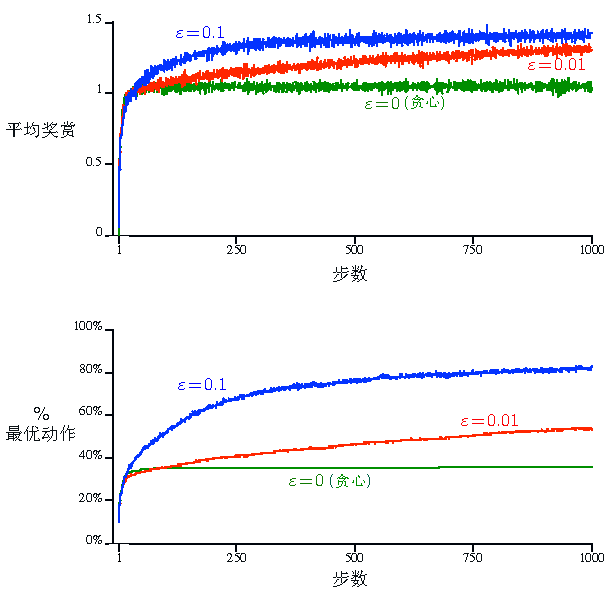
\includegraphics[width=.7\textwidth]{c2/img/figure2-2.pdf}
\caption{$\varepsilon$-贪心动作值方法在10-摇臂测试工具上的平均表现. 这些数据是对超过2000次使用不同赌博机问题的行程中的数值的平均. 所有的方法使用采样平均方法估计动作值.}\label{fig:2.2}
\end{figure}

$\varepsilon$-贪心方法对贪心方法的优势视任务而定. 例如, 假设奖赏的方差变得更大, 比如是10而不是1. 对于有更多噪声的奖赏, 代理需要更多的探索来发现最优动作, 那么$\varepsilon$-贪心方法的优势甚至会更大. 在另一方面, 如果奖赏的方差为0, 那么贪心方法在试过一次后就可以得知所有动作的真实值. 在这种情况下贪心方法可能是表现得最好的, 因为其立即发现了最优解, 然后不再做任何探索. 但如果我们弱化一些假设, 即使是在确定性<deterministic>\footnote{表示概率为1, 如上述的方差为0的情形, 与下述的(非)固定性在意义上不同}情况下, 探索也能很有优势. 例如, 假设赌博机问题是非固定性<nonstationary>的, 即动作的真实值会随时间变化. 在这种情况下, 即使有确定性这一性质的存在, 依然需要探索来保证没有一个非贪心动作变得比贪心动作更好. 就像我们在接下来的几章看到的那样, 非固定性情况在强化学习中最为常见. 即使潜在的任务是确定性与固定性的, 学习器也可能面临一组这样的任务, 其中每个任务都随着学习的进行和代理的决策策略的变化而随时间改变. 强化学习需要对探索与利用的平衡.

\begin{exer}[赌博机例子]
考虑一个$k = 4$的$k$-摇臂赌博机问题, 其中各个摇臂分别记为1, 2, 3, 4. 将一赌博机算法应用于该问题, 该算法使用$\varepsilon$-贪心动作选择与样本平均动作值估计方式, 且对所有的动作$a$, 初始估计值$Q_1(a) = 0$. 假设最开始的动作与奖赏序列为$A_1 = 1$, $R_1 = -1$, $A_2 = 2$, $R_2 = 1$, $A_3 = 2$, $R_3 = -2$, $A_4 = 2$, $R_4 = 2$, $A_5 = 3$, $R_5 = 0$. 其中有些时步$\varepsilon$情况发生了, 使得一个动作被随机选择. 在哪些时步中这一定发生了? 在哪些时步中可能发生了?
\end{exer}

\begin{exer}
在\figref{2.2}的比对中, 从长期来看, 哪种方法会在累积奖赏和选择最优动作的概率方面表现最佳? 该方法会比其他方法好多少? 请定量地表达你的观点.
\end{exer}

% ----------------------------------- sec2.4 ---------------------------------------------
\section{增量式实现}\label{sec:2.4}

我们至今讨论的动作值方法全都使用观察到的奖赏的样本均值来估计动作值. 我们现在转向``这些平均值应该怎样才能以高效的方式被计算出来''这一问题, 更具体地说, 怎样以常数的内存使用与每一时步中常数的计算时间计算出来. 

为了简化标记, 我们将专注于单个动作上. 让$R_i$表示在第$i$次选择该动作后接收到的奖赏, 并以$Q_n$表示在选择了$n - 1$次该动作后其估计值, 现在我们可以简单地将$Q_n$写作
\begin{equation*}
Q_n \doteq \frac{R_1 + R_2 + \dots + R_{n - 1}}{n - 1}.
\end{equation*}
最显而易见的实现方式就是维持对所有接收到的奖赏的记录, 然后每当需要估计值的时候就计算上方的等式. 然而, 以这种方式实现的话, 对内存与计算时间的需求会随着越来越多的奖赏被观察到而逐步增大. 每一个新观察到的奖赏都会需要额外的内存来存储, 需要额外的计算时间来计算分子中的和.

就像你怀疑的那样, 这事实上并不是必需的. 很简单就能发明增量式地更新均值的公式, 且只需要极小的、常数的计算时间来处理每个新奖赏. 给定$Q_n$和第$n$次的奖赏$R_n$, 所有$n$个奖赏的新的均值可以使用下式计算
\begin{equation}\label{eq:2.3}
\begin{aligned}[b]
Q_{n + 1} &= \frac{1}{n} \sum_{i = 1}^n R_i \\
&= \frac{1}{n} \left( R_n + \sum_{i = 1}^{n - 1}R_i \right) \\
&= \frac{1}{n} \left( R_n + (n - 1) \frac{1}{n - 1} \sum_{i = 1}^{n - 1}R_i \right) \\
&= \frac{1}{n} \left( R_n + (n - 1) Q_n \right) \\
&= \frac{1}{n} \left( R_n +n Q_n - Q_n \right) \\
&= Q_n + \frac{1}{n} \left[ R_n - Q_n \right],
\end{aligned}
\end{equation}
上述的等式甚至在$n = 1$时也成立, 即$Q_2 = R_1$, 对任意$Q_1$均成立. 这一实现方式只需要存储$Q_n$和$n$的内存, 以及对每个新奖赏使用\eqref{eq:2.3}的极小的计算时间.

更新规则\eqref{eq:2.3}属于一种在全书中经常出现的更新形式. 这一一般形式为
\begin{equation}\label{eq:2.4}
\begin{aligned}[b]
\text{新估计值} &\leftarrow \text{旧估计值} + \text{步长} [\text{目标} - \text{旧估计值}] \\
(NewEstimate &\leftarrow OldEstimate + StepSize [Target - OldEstimate])
\end{aligned}
\end{equation}
表达式$[\text{目标} - \text{旧估计值}]$是估计中的\emph{误差}<error>. 通过向``目标''靠近来减小该误差. 假定上, 目标预示着希望的移动方向, 虽然这可能是有噪声的. 例如在前述的情形中, 目标就是第$n$次奖赏.

\begin{pcbox}{一个简单的赌博机算法}{!ht}
\pcind[0] 初始化, for $a = 1$ to $k$: \\
\pcind[1] $Q(a) \leftarrow 0$ \\
\pcind[1] $N(a) \leftarrow 0$ \\
\pcind[0] Loop forever:\\
\pcind[1] $A \leftarrow \begin{cases} \targmax_a Q(a) &\text{以}1-\varepsilon\text{的概率(若多个最值, 随意选择)}\\ \text{一个随机动作} & \text{以}\varepsilon \text{的概率} \end{cases}$ \\
\pcind[1] $R \leftarrow bandit(A)$ \\
\pcind[1] $N(A) \leftarrow N(A) + 1$ \\
\pcind[1] $Q(A) \leftarrow Q(A) + \frac{1}{N(A)}[R - Q(A)]$
\end{pcbox}

注意在增量式方法\eqref{eq:2.3}中步长参数会随时间变化. 在处理对动作$a$的第$n$次奖赏时, 该方法使用的步长参数为$\frac{1}{n}$. 在本书中我们将步长参数记为$\alpha$, 或更为一般的, 记为$\alpha_t(a)$.

% ref warning
使用增量式计算的样本均值与$\varepsilon$-贪心动作选择的完整赌博机算法的伪代码展示在了前一页的方框内. 函数$bandit(a)$假定为以动作为参数, 返回相应奖赏的函数.


% ----------------------------------- sec2.5 ---------------------------------------------
\section{追踪非固定性问题}\label{sec:2.5}

我们至今讨论的平均方法可以适用于固定性赌博机问题, 即奖赏的概率分布不会随时间变化的赌博机问题. 就像之前指出的那样, 实际上我们经常遇到非固定性的强化学习问题. 在这种情况下, 相对于较早的奖赏, 将更多的权重给予较近的奖赏是很有意义的. 最为流行的、能做到这一点的方法之一就是使用固定的步长参数. 例如, 对过去的$n - 1$次奖赏的平均, $Q_n$, 其增量式更新规则\eqref{eq:2.3}可以改写为
\begin{equation}\label{eq:2.5}
Q_{n + 1} \doteq Q_n + \alpha [R_n - Q_n],
\end{equation}
其中步长参数$\alpha \in (0, 1]$, 为一常数. 这使得了$Q_{n + 1}$成为了对过去奖赏与初始估计值$Q_1$的加权平均:
\begin{equation}\label{eq:2.6}
\begin{aligned}[b]
Q_{n + 1} &= Q_n + \alpha [R_n - Q_n] \\
&= \alpha R_n + (1 - \alpha) Q_n \\
&=  \alpha R_n + (1 - \alpha) [\alpha R_{n - 1} + (1 - \alpha)Q_{n - 1}] \\
&=  \alpha R_n + (1 - \alpha) \alpha R_{n - 1} + (1 - \alpha)^2 Q_{n - 1} \\
&=  \alpha R_n + (1 - \alpha) \alpha R_{n - 1} + (1 - \alpha)^2 \alpha R_{n - 2} + \dots + (1 - \alpha)^{n - 1} \alpha R_1 + (1 - \alpha)^n Q_1 \\
&= (1 - \alpha)^n Q_1 + \sum_{i = 1}^n \alpha (1 - \alpha)^{n - i} R_i.
\end{aligned}
\end{equation}
我们将此称为加权平均, 因为权重之和$(1 - \alpha)^n + \sum_{i = 1}^n \alpha (1 - \alpha)^{n - i} = 1$, 读者可以自行证明. 请注意给予奖赏$R_i$的权重$\alpha (1 - \alpha)^{n - i}$取决于在多少次奖赏前该奖赏被观察到, 即$n - 1$的值. $1 - \alpha$的值小于1, 因此给予$R_i$的权重会随着与迄今间隔的奖赏次数增加而减少. 事实上, 因为以$1 - \alpha$为底的指数因子的存在, 该权重会指数衰减(如果$1 - \alpha = 0$, 那么所有的权重都集中于最新的奖赏$R_n$, 因为依照惯例$0^0 = 1$). 所以, 这有时也被称为\emph{指数新近加权平均}<exponential recency-average>.

有时, 在每一步都改变步长参数可以提供便利. 令$\alpha_n (a)$表示用于处理第$n$次选择动作$a$后所收到奖赏的步长参数. 如我们之前所说, 若$\alpha_n (a) = \frac{1}{n}$, 即为采样平均方法, 而依据大数定理其确保能收敛到真实的动作值. 但理所当然, 不是所有的序列选择${\alpha_n(a)}$都确保能收敛. 一个随机逼近理论<stochastic approximation theory>中的著名结论, 为我们提供了能以1的概率保证收敛的条件:
\begin{equation}\label{eq:2.7}
\sum_{n = 1}^\infty \alpha_n(a) = \infty  \; \text{且} \; \sum_{n = 1}^\infty \alpha_n^2(a) < \infty
\end{equation}
我们需要第一个条件来保证这些步长对``最终克服初始条件或随机波动的影响''而言足够大. 第二个条件确保最终步长变得足够小以确保收敛. 

请注意采样平均的情形, 即$\alpha_n(a) = \frac{1}{n}$, 满足上述两个条件; 而步长恒定的情形, 即$\alpha_n(a) = \alpha$, 并非如此. 对后者而言, 其并不能满足第二个条件, 这意味着估计值不会完全收敛, 而是继续随新收到的奖赏变化. 就像我们之前提到过的那样, 这事实上正是非固定性环境所需要的, 而实际上非固定性问题在强化学习中是最为常见的. 此外, 满足条件\eqref{eq:2.7}步长参数序列常常收敛得非常缓慢或需要大量的调参来获得令人满意的收敛速率. 虽然满足上述收敛条件的步长参数序列常常用于理论研究中, 但极少用于实际应用或实证研究中.

\begin{exer}
如果步长参数$\alpha_n$不是常数, 那么估计值$Q_n$为对之前所收到奖赏的加权平均, 且权重与\eqref{eq:2.6}给出的不同. 那么类比于\eqref{eq:2.6}, 怎么使用步长参数序列, 来表示一般情形下的各个已收到的奖赏的权重?
\end{exer}

\begin{exer}
设计并实现一个实验, 来解释样本平均方法在处理非固定性问题时所面临的困境. 可以使用10-摇臂测试工具的修改版本, 其中所有的$q_*(a)$初始值相同, 然后独立地随机变动(例如在每一步, 向各个$q_*(a)$添加采样自均值为0且标准差为0.01的正态分布的增量). 然后为以下两种动作值方法绘制类似\figref{2.2}的图表: 其一使用增量式计算的样本平均法; 其二使用恒定步长参数$\alpha = 0.1$. 此外, 令$\varepsilon = 0.1$, 并且使用更长的行程, 例如10,~000步.
\end{exer}

% ----------------------------------- sec2.6 ---------------------------------------------
\section{乐观初始值}\label{sec:2.6}

我们至今讨论的所有方法或多或少依赖于初始的动作值的估计值, $Q_1(a)$. 用统计学的术语来说, 这些方法因初始的估计值产生了偏差<bias>. 对于样本平均方法来说, 当所有的动作都被选择了一次后偏差就消失了; 但对$\alpha$值恒定的方法来说, 这一偏差会永远存在, 但会随时间逐步减小, 正如\eqref{eq:2.6}所示. 在实际应用中, 这类偏差常常并不成问题, 反而有时还很有帮助. 其负面影响是初始值实际上变成了一组必须由用户选择的参数, 要是能将它们都设为0的话该多好. 其正面影响是提供了一种简单的方式, 来应用关于预期的奖赏值的水平的先验知识.

初始动作值也可以以一种简单的鼓励探索的方式来使用. 如果我们在10-摇臂测试工具中, 不是将初始动作值都设为0, 而是将其都设为$+5$. 我们还记得在该问题中$q_*(a)$是从均值为0且方差为1的正态分布中采样得到的. 因此$+5$的初始估计值是极为乐观的. 但这份乐观鼓励了动作值方法去探索. 无论开始时选择了哪个动作, 收到的奖赏都低于初始估计值; 学习器因此对收到的奖赏感到``失望'', 转而选择别的动作. 结果就是所有的动作都在估计值收敛前被选择了数次. 即使一直选择贪心动作, 强化学习系统事实上也做了大量的探索.

\figref{2.3}展示了$Q_1(a) = +5$的贪心方法在10-摇臂测试工具上的表现. 作为对比, $Q_1(a) = 0$的$\varepsilon$-贪心方法也展示在了图中. 最开始, 乐观方法表现得比$\varepsilon$-贪心方法差, 但因为乐观方法的探索随时间流逝减少, 因此最终乐观方法的表现好于$\varepsilon$-贪心方法. 我们将这一鼓励探索的技术称为\emph{乐观初始值}<optimistic initial values>. 我们将其视作一个在固定性问题上可以表现得非常高效的小技巧, 但其远不能成为一个通用的有效鼓励探索的方法. 例如, 其不适宜于非固定性问题, 因为其对探索的驱动本质上是暂时的. 如果任务变化并对探索产生了新的需求, 那么这一方法就无能为力了. 事实上, 以任何特定的方式关注于初始值的方法都对一般的非固定性问题无能为力. 时间上的开端只会出现一次, 因此我们不应该对开端过分关注. 这一评判也适用于样本平均方法, 其也将时间上的开端作为特别事件, 并以均等的权重来平均所有的后续奖赏. 话虽如此, 所有这些方法都很简单, 且这些方法中的一个或多个的组合常常对实际应用而言足够了. 在本书的余下部分中我们将频繁使用这些简单的探索技术.

\begin{figure}[ht]
\centering
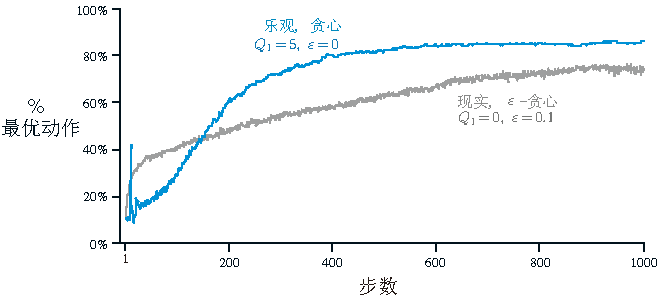
\includegraphics[width=.75\textwidth]{c2/img/figure2-3.pdf}
\caption{乐观的动作值初始估计在10-摇臂测试工具上的表现. 两种方法都使用了恒定步长参数$\alpha = 0.1$.}\label{fig:2.3}
\end{figure}

\begin{exer}[神秘的尖峰]
\figref{2.3}中显示的结果应该是很可靠的, 因为其为2000个独立的、随机选择的10-摇臂赌博机问题上的结果的平均. 那么在乐观方法的曲线的开始部分为什么会有震荡与尖峰? 换句话说, 是什么使得这一方法在特定的较早时步中, 从平均的意义上说表现得特别好或特别差?
\end{exer}

\begin{exer}[无偏的恒定步长技巧]
在本章的多数部分中我们使用了样本均值来估计动作值, 因为样本平均法不会产生如恒定步长方法所拥有的初始偏差(具体见导出\eqref{eq:2.6}的分析). 然而, 样本平均方法可能不是一个完全令人满意的解决方案, 因为其在非固定性问题上表现不佳. 有没有可能避免恒定步长带来的偏差又保持其在非固定性问题上的优势? 一种方法是使用如下步长
\begin{equation}\label{eq:2.8}
\beta_n \doteq \alpha / \bar{o}_n,
\end{equation}
来处理第某一动作带来的第$n$次的奖赏, 其中$\alpha > 0$, 是常规的恒定步长, 而$\bar{o}_n$为从0开始逐步靠近1的序列:
\begin{equation}\label{eq:2.9}
\bar{o}_n = \bar{o}_{n - 1} + \alpha (1 - \bar{o}_{n - 1}), \; \text{对} n \geq 0 \text{, 且其中} \bar{o}_0 \doteq 0
\end{equation}
做出如\eqref{eq:2.6}中的分析来证明$Q_n$是无初始偏差的指数新近衰减平均.
\end{exer}

% ----------------------------------- sec2.7 ---------------------------------------------
\section{上置信界动作选择}\label{sec:2.7}

因为对动作值估计的准确度的不确定性存在, 所以需要进行探索. 贪心动作是当前看上去最好的动作, 但其他动作中的一些可能事实上更好. $\varepsilon$-贪心动作选择强制使得非贪婪动作被选择, 但这一过程对各个动作是不加区分的, 即使是接近贪心或特别不确定的动作也不被偏好. 对非贪心动作来说, 将其估计值离成为最大值的距离与估计值中的不确定性考虑在内, 由此判断各个非贪心动作成为最优动作的潜力, 然后根据这个潜力进行动作动作选择显然是更好的. 一种能做到这一点的高效方式就是由下式进行动作选择
\begin{equation}\label{eq:2.10}
A_t \doteq \underset{a}{\operatorname{argmax}} \left[ Q_t(a) + c \sqrt{\frac{\ln t}{N_t(a)}} \;\right],
\end{equation}
其中$\ln t$表示$t$的自然对数($e \approx 2.71828$的该数次幂等于$t$), $N_t(a)$表示在时间$t$之前动作$a$被选择的次数(\eqref{eq:2.1}中的分母), 以及常数$c > 0$控制了探索的程度. 如果$N_t(a) = 0$, 那么$a$被认为是最优动作.

如上所述的\emph{上置信界}<upper confidence bound, UCB>动作选择的观念为: 式中的根号项是对$a$的估计值的不确定度或方差. 欲寻求最大值的项\footnote{即$\dargmax_a$右侧的量, 译者注}, 是动作$a$可能的真实值的上界的一种, 其中由$c$决定置信水平. 每当$a$被选择时, 不确定性可以被认为是减少了: $N_t(a)$增加, 因为其出现在分母中, 所以不确定性项减小了. 在另一方面, 每当除$a$之外的动作被选择, $t$增加而$N_t(a)$保持不变; 因为$t$出现在分子中, 所以对不确定性的估计增加了. 自然对数的使用意味着增长的速率逐渐变慢, 但其值依然会趋近于无穷大; 所有的动作都会被选择, 但有较低的估计值或已经被频繁选择过的动作, 将会随时间推移减少被选择的频率. 在10-摇臂测试工具上使用UCB的结果如\figref{2.4}所示. 像图中所展示的那样, UCB常常表现得很好, 但相比于$\varepsilon$-贪心而言, 其更难以从赌博机问题拓展到书中余下部分中的, 更为一般的强化学习情形. 其中的一个困难之处就是对非固定性问题的处理——需要比\secref{2.5}中所呈现的更为复杂的方法. 另一个困难之处出现于对巨大状态空间的处理, 特别是当使用了如本书\partref{2}所述的函数近似方法时. 在这些更为复杂的情形下, UCB动作选择通常是不理想的. 

\begin{figure}[ht]
\centering
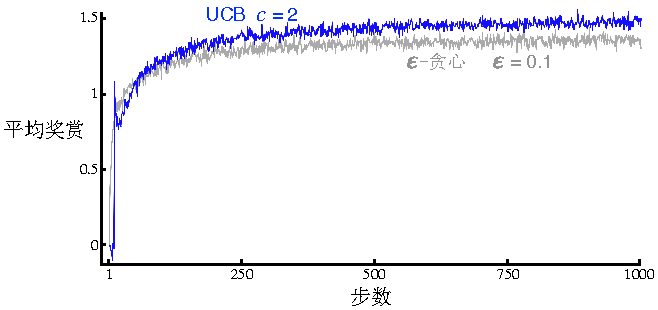
\includegraphics[width=.75\textwidth]{c2/img/figure2-4.pdf}
\caption{UCB动作选择在10-摇臂测试工具中的平均表现. 如图所示, 除了UCB从尚未尝试过的动作中随机进行选择的起始$k$步外, UCB通常表现得比$\varepsilon$-贪心动作选择好.}\label{fig:2.4}
\end{figure}

\begin{exer}[UCB尖峰]
在\figref{2.4}中UCB算法的表现在第11步时有一个明显的尖峰. 为什么会这样? 请注意, 为了使答案完全令人满意, 其需要从``为什么奖赏在第11步增加了?'', 以及``为什么奖赏又在后续的几步中减小了?''这两个方面进行解释. 提示: 如果$c = 1$, 那么尖峰将更矮.
\end{exer}

% ----------------------------------- sec2.8 ---------------------------------------------
\section{梯度赌博机算法}\label{sec:2.8}

在本章的之前部分, 我们已经学习了对动作值进行估计, 然后使用估计值来选择动作的多种方法. 这常常是一种好的途径, 但并不是唯一的途径. 在本节中, 我们将考虑如何为每一个动作$a$学得各自实数型的\emph{偏好}<pautoreference>, 我们将其记为$H_t(a)$. 偏好值越高, 那么对应的动作越常被采用, 但是偏好不能使用奖赏的观念来理解. 只有一个动作相较于另一个动作的相对偏好值是有意义的; 如果我们将所有动作的偏好值加上1000, 各个动作被选择的概率仍然保持不变, 其中概率是由如下的\emph{soft-max分布}(也称为Gibbs分布或Boltzmann分布)决定的:
\begin{equation}\label{eq:2.11}
\Pr\{A_t = a\} \doteq \frac{e^{H_t(a)}}{\sum_{b = 1}^{k} e^{H_t(b)}} \doteq \pi_t(a),
\end{equation}
这里我们引入一种实用的新标记$\pi_t(a)$, 来表示在时步$t$采取动作$a$的可能性. 起始时, 所有动作的偏好值都是相等的(例如对所有的a来说, $H_1(a) = 0$), 因此所有动作都有相同的被选择的概率.

\begin{exer}
证明在只有两个动作的情况下, soft-max分布, 和统计学及人工神经网络中常用的logistic或sigmoid函数给出的分布是等价的.
\end{exer}

基于随机梯度上升<stochastic gradient ascent>, 可以自然地得到这一设定下的学习算法. 在每一步时, 在选择动作$A_t$并收到奖赏$R_t$后, 动作偏好值使用下式进行更新:
\begin{equation}\label{eq:2.12}
\begin{aligned}[b]
H_{t + 1}(A_t) &\doteq H_t(A_t) + \alpha (R_t - \bar{R}_t)(1 - \pi_t(A_t)), &&\text{且} \\
H_{t + 1}(a) &\doteq H_t(a) - \alpha(R_t - \bar{R}_t) \pi_t(a), &&\text{对所有的}a \neq A_t,
\end{aligned}
\end{equation}
其中$\alpha > 0$, 为步长参数, 且$\bar{R}_t \in \mathbb{R}$, 为时步$t$及之前的所有奖赏的平均, 可以如\secref{2.4}(如果问题是非固定性的话, 那么如\secref{2.5})中所述的那样进行增量式的计算. $\bar{R}_t$这一项是作为比较奖赏的基准线的. 如果奖赏高于基准线, 那么将来采取动作$A_t$的概率将增加; 反之如果奖赏低于基准线, 那么概率将减小. 而未被选择的动作的概率朝相反方向移动.

\begin{figure}[!ht]
\centering
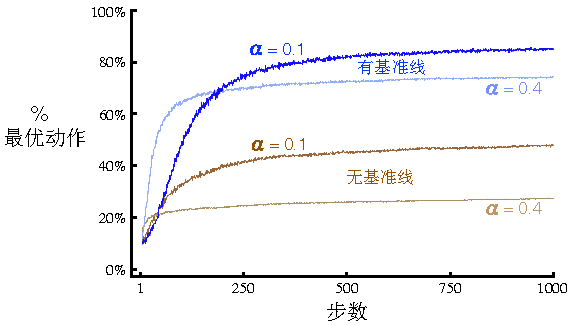
\includegraphics[width=.7\textwidth]{c2/img/figure2-5.pdf}
\caption{在$q_*(a)$接近+4而非0的10-摇臂测试工具上, 有无奖赏基准线的梯度赌博机算法的平均表现.}\label{fig:2.5}
\end{figure}

\figref{2.5}展示了梯度赌博机算法在10-摇臂测试工具的变体上的结果, 该变体中真实的期望奖赏是从一均值为$+4$而非0(方差和从前一样为1)的正态分布中采样获得的. 所有奖赏的同时增加对梯度赌博机算法绝对没有影响, 因为奖赏的基准线会立即适应到新的水平上. 但如果基准线被省略了(即如果\eqref{eq:2.12}中的$\bar{R}_t$恒取0), 那么其性能将如图中所示的那样急剧退化.

\FloatBarrier
\begin{mathbox}{作为随机梯度上升的梯度赌博机算法}
我们可以将梯度赌博机算法理解为梯度上升的概率性近似, 来获得更深入的理解. 在典型的\emph{梯度上升}<gradient ascent>中, 各个动作的偏好值$H_t(a)$将会正比于增量在表现<performance>上的效果而增加:
\begin{equation}\label{eq:2.13}
H_{t + 1}(a) \doteq H_t(a) + \alpha \frac{\partial \mathbb{E}[R_t]}{\partial H_t(a)},
\end{equation}
其中表现上的度量即为奖赏的期望值:
\begin{equation*}
\mathbb{E}[R_t] = \sum_x \pi_t(x) q_*(x),
\end{equation*}
且对增量的效果的度量为: 表现上的度量相对于动作偏好值的\emph{偏导数}. 当然, 因为假设上我们不知道$q_*(x)$, 所以不可能在现有情况下实现典型的梯度上升, 但事实上从期望值的角度看, 算法\eqref{eq:2.12}中的更新等同于\eqref{eq:2.13}中的更新, 这使得前者成为了\emph{随机梯度上升}方法的实例. 证明这一点的推导只需要初等的微积分知识, 但是需要花费数步. 首先让我们更近地看一看表现的梯度:
\begin{equation*}
\begin{aligned}[b]
\frac{\partial \mathbb{E}[R_t]}{\partial H_t(a)} &= \frac{\partial}{\partial H_t(a)} \left[ \sum_x \pi_t(x) q_*(x) \right] \\
&= \sum_x q_*(x) \frac{\partial \pi_t(x)}{\partial H_t(a)} \\
&= \sum_x (q_*(x) - B_t) \frac{\partial \pi_t(x)}{\partial H_t(a)},
\end{aligned}
\end{equation*}
其中$B_t$被称为\emph{基准线}, 可以为任意不依赖于$x$的标量. 我们可以在不改变等号的情况下加入基准线项, 这是因为所有动作上梯度值的和为0, 即$\sum_x \frac{\partial \pi_t(x)}{\partial H_t(a)} = 0\;$——如果$H_t(a)$改变的话, 一些动作被选择的概率增加而一些减小, 但概率的改变量之和为0, 因为概率的和永远为1.

接下来我们令上一式中和的每一项都乘以$\pi_t(x) / \pi_t(x)$:
\begin{equation*}
\frac{\partial \mathbb{E}[R_t]}{\partial H_t(a)}  = \sum_x \pi_t(x) (q_*(x) - B_t) \frac{\partial \pi_t(x)}{\partial H_t(a)} / \pi_t(x).
\end{equation*}
现在这一等式正符合期望的形式, 即等式中有在随机变量$A_t​$的所有可能取值之上的和, 以及取这些值的概率这一乘积项. 因此
\begin{equation*}
\begin{aligned}[b]
\phantom{\frac{\partial \mathbb{E}[R_t]}{\partial H_t(a)}}
&= \mathbb{E} \left[ (q_*(A_t) - B_t) \frac{\partial \pi_t(A_t)}{\partial H_t(a)} / \pi_t(A_t) \right]\\
&= \mathbb{E} \left[ (R_t - \bar{R}_t) \frac{\partial \pi_t(A_t)}{\partial H_t(a)} / \pi_t(A_t) \right] 
\end{aligned}
\end{equation*}
其中我们选择了基准线$B_t = \bar{R}_t​$, 并将$q_*(A_t)​$替换为$R_t​$, 可以这么做的原因是$\mathbb{E}[R_t \mid A_t] = q_*(A_t)​$. 等等我们会证明$\frac{\partial \pi_t(x)}{\partial H_t(a)} = \pi_t(x)(\mathbbm{1}_{a = x} - \pi_t(a))​$, 该式中如果$a = x​$那么$\mathbbm{1}_{a = x}​$为1, 反之为0. 先假设这一点是成立的, 那么我们有
\begin{equation*}
\begin{aligned}[b]
\phantom{\frac{\partial \mathbb{E}[R_t]}{\partial H_t(a)}}
&= \mathbb{E} \left[ (R_t - \bar{R}_t) \pi_t(A_t) (\mathbbm{1}_{a = A_t} - \pi_t(a)) / \pi_t(A_t) \right] \\
&= \mathbb{E} \left[ (R_t - \bar{R}_t) (\mathbbm{1}_{a = A_t} - \pi_t(a)) \right] 
\end{aligned}
\end{equation*}
回想下, 我们想要将表现的梯度, 写作我们可以在每一步采样的某物的期望值, 而我们已经做到了这一点, 然后我们可以正比于样本值对偏好值进行更新. 将上式中的期望值替换为样本值, 并带入\eqref{eq:2.13}中, 我们可以得到:
\begin{equation*}
H_{t + 1}(a) = H_t(a) + \alpha (R_t - \bar{R}_t)(\mathbbm{1}_{a = A_t} - \pi_t(a)), \text{ 对所有的}a
\end{equation*}
然后你会发现上式和我们原先的算法\eqref{eq:2.12}相等.

余下的部分即为证明我们的假设$\frac{\partial \pi_t(x)}{\partial H_t(a)} = \pi_t(x)(\mathbbm{1}_{a = x} - \pi_t(a))$. 回想下导数的商公式:
\begin{equation*}
\frac{\partial}{\partial x}\left[ \frac{f(x)}{g(x)} \right] = \frac{\frac{\partial f(x)}{\partial x}g(x) - f(x)\frac{\partial g(x)}{\partial x}}{g(x)^2}.
\end{equation*}
使用这一点, 我们可以得到:
\begin{equation*}
\begin{aligned}[b]
\frac{\partial \pi_t(x)}{\partial H_t(a)} 
&= \frac{\partial}{\partial H_t(a)} \pi_t(x) \\
&= \frac{\partial}{\partial H_t(a)} \left[ \frac{e^{H_t(x)}}{\sum_{y = 1}^k e^{H_t(y)}} \right] \\
&= \frac{\frac{\partial e^{H_t(x)}}{\partial H_t(a)} \sum_{y = 1}^k e^{H_t(y)} - e^{H_t(x)} \frac{\partial \sum_{y = 1}^k e^{H_t(y)}}{\partial H_t(a)}} {\left( \sum_{y = 1}^k e^{H_t(y)}\right)^2 }  &\text{(通过商公式)}\\
&= \frac{\mathbbm{1}_{a = x} e^{H_t(x)} \sum_{y = 1}^k e^{H_t(y)} - e^{H_t(x)} e^{H_t(a)}}{\left( \sum_{y = 1}^k e^{H_t(y)}\right)^2} &\text{(因为} \frac{\partial e^x}{\partial x} =e^x \text{)} \\
&= \frac{\mathbbm{1}_{a = x} e^{H_t(x)}}{\sum_{y = 1}^k e^{H_t(y)}} - \frac{e^{H_t(x)} e^{H_t(a)}}{\left( \sum_{y = 1}^k e^{H_t(y)}\right)^2} \\
&= \mathbbm{1}_{a = x} \pi_t(x) - \pi_t(x) \pi_t(a) \\
&= \pi_t(x)\left( \mathbbm{1}_{a = x} - \pi_t(a) \right).  &\text{得证}
\end{aligned}
\end{equation*}

我们刚刚证明了梯度赌博机算法的更新的期望值等于期望奖赏的梯度, 所以此算法为随机梯度下降的实例. 这保证了算法有鲁棒的收敛性质.

请注意, 对于奖赏基准线而言, 除了其不能依赖于所选择的动作外, 我们没有更多的要求. 例如, 我们可以将其值设为0, 也可以将其值设为1000, 但梯度赌博机算法依然是随机梯度下降的实例. 基准线的选择不影响算法中期望的更新, 但其影响更新的方差, 因此影响了收敛的速率(例如, 如\figref{2.5}所示). 将其设为奖赏的均值可能不是最好的, 但这一选择既简单又在实际使用中很表现得很好. 
\end{mathbox}

% ----------------------------------- sec2.9 ---------------------------------------------
\section{关联搜索(上下文相关赌博机)}\label{sec:2.9}

在本章的前面部分, 我们只考虑了非关联任务, 即不需要将不同的动作与不同的情形相关联的任务. 在这种任务中, 如果任务是固定性的, 那么学习器试图寻找单个的最佳动作; 如果任务是非固定性的, 那么学习器试图随时间的变动追踪最佳的动作. 然而在一般的强化学习任务中, 情形的数量不止一个, 且目标是学得一个策略——一个从情形到该情形下的最佳动作的映射. 我们将简短地讨论将非关联任务拓展到关联任务的最简单的方式, 以为完整的强化学习问题做准备.

举个例子, 假如有数个不同的$k$-摇臂赌博机任务, 并且在每一步随机地遇到其中的某一个. 因此在每一步赌博机任务都可能会变动. 这看上去像一个简单的、非固定性的$k$-摇臂赌博机任务, 只是其中真实的动作值在每一步都会随机发生变化. 你可以尝试使用本章前面部分所述的、处理非固定性任务的方法, 但除非真实的动作值变动得很缓慢, 否则这些方法无法表现得好. 现在假设, 当某一个赌博机任务被选中时, 你被给予了关于赌博机身份(而非动作值)的区分线索. 比如你面对着一个现实中的老虎机, 当其改变各个动作值时其外表的颜色也会发生变化. 现在你可以学得一个策略, 将由颜色标识的任务, 同该任务下最佳的动作关联起来——例如, 如果为红色, 选择第1条摇臂; 如果为绿色, 选择第2条摇臂. 在正确的策略下, 这常常可以做得远比在缺失赌博机的辨别信息的条件时好. 

这是一个\emph{关联搜索}<associative search>任务的例子, 其之所以被这么称呼, 是因为其既涉及到使用试错来\emph{搜索}最佳的动作, 又涉及到将最佳的动作同各自的情形进行\emph{关联}. 关联搜索任务常在文献中被称为\emph{上下文相关赌博机}<contextual bandit>. 关联搜索任务介于$k$-摇臂赌博机问题和完整的强化学习问题之间. 从其``涉及到学得一个策略''这一点来看, 其类似于完整的强化学习问题; 但从``每一个动作仅影响当前的奖赏''这一点来看, 其又类似于本书中的$k$-摇臂赌博机问题版本. 如果动作除了能影响奖赏外, 也能影响\emph{下一状态}, 那么就得到了完整的强化学习任务. 我们将在下一章中呈现完整的强化学习问题, 并在本书的余下部分中考虑其各个分支.

\begin{exer}
假设你面临着真实动作值在每一步随机变动的2-摇臂赌博机任务. 特别地, 假设在每一步, 以0.5的概率动作1和动作2的真实值分别为0.1和0.2(情形A), 以0.5的概率动作1和动作2的真实值分别为0.9和0.8(情形B). 如果你在每一步不能分辨出所面临的情形, 那么你能期望的最高奖赏是多少? 怎么达到这一点? 如果假设在每一步你都被告知了你所面临的是情形A还是情形B(然而你仍不知道真实的动作值). 这就成了一个关联搜索任务. 那么你梦期望的最高奖赏是多少? 怎么达到这一点?
\end{exer}

% ----------------------------------- sec2.10 ---------------------------------------------
\section{总结}\label{sec:2.10}

我们已在本章中呈现了几种平衡探索与利用的简单方式. $\varepsilon$-贪心方法在一小部分时间中随机选择动作, 而UCB方法确定性地进行动作选择, 但通过巧妙地支持迄今为止采样次数较少的动作来实现探索. 梯度赌博机算法不是对动作值进行估计, 而是对动作偏好进行估计, 并使用soft-max分布, 以一种分级的、概率性的方式来向更偏好的动作倾斜. 对估计值进行乐观的初始化这一简单的权宜之计, 使得即使是贪心方法也会进行大量探索.

\vspace{1em}
\begin{figure}[ht]
\centering
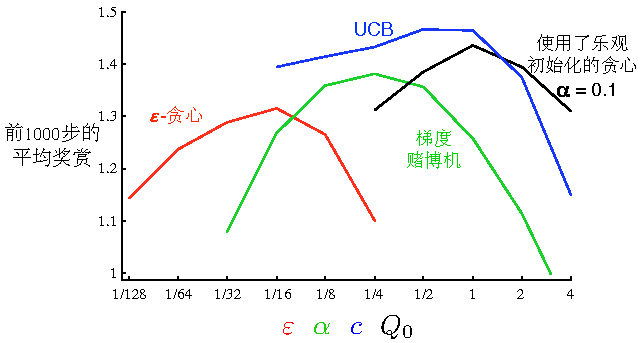
\includegraphics[width=.75\textwidth]{c2/img/figure2-6.pdf}
\caption{一份对本章中出现的各个方法的参数审视. 每一点都是特定算法与特定参数下的, 1000步奖赏的均值.}\label{fig:2.6}
\end{figure}

那么很自然地就要问这些方法中哪一个是最好的. 虽然这个问题整体上而言很难回答, 但我们显然可以在贯穿了本章的10-摇臂测试工具上使用各个方法, 并比较各自的表现. 一个困难之处是各个方法都有一个参数; 为了得到一个有意义的比较, 我们不得不将各个方法的表现作为自身参数的函数来对待. 至今为止, 我们所作的图展示了每一算法与每一参数下, 随时间变化的学习过程, 来产生在该算法与该参数设定下的\emph{学习曲线}<learning curve>. 如果我们为所有算法的所有参数设定绘制学习曲线, 那么所绘制的图将过于复杂与臃肿, 而无法产生清晰的比较. 作为代替, 我们可以使用其1000步上的平均值来代替完整的学习曲线; 这一值同学习曲线下的面积成正比. \figref{2.6}展示了本章中各个算法的这一度量, 且每一方法的度量都是各自参数的函数, 各参数使用如x轴所示的统一的标度. 这类图被称为\emph{参数审视}<parameter study>. 请注意参数值以2为因子倍增, 以对数的标度进行呈现. 也请注意各个算法的表现中极具特色的倒U形: 所有的方法在使用居中的参数值时表现最好, 即参数值既不能太大, 也不能太小. 在评估一个方法时, 我们不仅需要关注其在最佳参数设定下的表现, 也需要关注其对参数值的敏感程度. 所有的这些算法都相当不敏感, 都在一个量级的参数范围内都表现得很好. 总体而言, 在这个问题上UCB看上去表现最佳.

虽然都很简单, 但在我们看来本章中呈现的这些方法都可以算是先进水准. 虽然有更加精细的方法, 但对我们真正关注的完整强化学习问题而言, 其复杂性与所作的假设使得其不切实际. 从\chapref{5}开始, 我们将呈现用于解决完整强化学习问题的学习方法, 这些方法中就部分使用了本章中探讨的简单方法.

虽然本章中探讨的方法可能是我们目前所能做到的最好的, 但这些远不是``平衡探索与利用''这一问题的令人完全满意的解决方案.

一种经过透彻研究的, 用于平衡$k$-摇臂赌博机问题中的探索与利用的方法, 是计算一种被称为\emph{基廷斯指数}<Gittins index>的特殊动作值. 在一些重要的特殊情形下,  其在计算上易于处理, 并且可以直接计算出最优解, 但是其需要关于问题先验分布的完整知识, 而这些知识我们通常假设为是无法得到的. 此外, 无论是此方法的理论, 还是其计算上的易处理性, 都无法泛化到我们在本书的余下部分中考虑的完整强化学习问题上.

基廷斯指数方法是\emph{贝叶斯}<Bayesian>方法的一个实例. 贝叶斯方法会假设一个已知的在动作值上的初始分布, 然后在每一步后即更新该分布(假设真实的动作值是固定性的). 一般而言, 对更新的计算十分复杂,  但对于一些特定的分布(称为共轭先验<conjugate prior>)而言, 计算较为简单. 进行更新之后, 一种可行的手段是, 在每一步根据各个动作成为最优动作的后验概率来进行动作选择. 这一方法有时也被称为\emph{后验采样}<posterior sampling>或\emph{汤普森采样}<Thompson sampling>, 其通常和本章之前呈现的无分布方法<distribution-free method>中最好的那些在表现上类似.

在贝叶斯设定下, 即使想要计算探索与利用之间的\emph{最佳}平衡也是可能的. 我们可以为每一个可能的动作, 计算其所有可能的立即奖赏的概率, 以及作为结果的关于动作值的后验分布. 这一以上述方式不断行进的分布, 成为了该问题的\emph{信息状态}<information state>. 给定一定的步数, 例如1000步, 我们可以考虑所有可能的动作, 所有可能的作为结果的奖赏, 所有可能的下一动作, 所有的下一奖赏, 以此类推直到第1000步. 在这样的假设下, 所有可能的事件链的奖赏与概率都可以被确定, 我们只需要选择最佳的即可. 但是可能性树会急剧生长, 即使只有两种动作与两种奖赏, 树也会有$2^{2000}$个树叶.一般而言, 要真正进行如此大量的计算是不切实际的, 但是也许有高效的近似方式. 这一方法实际上将赌博机问题转换为了完整强化学习问题的实例. 最后, 也许我们能够使用\partref{2}中介绍的近似强化学习方法来获得这个最优解. 但这属于一个研究的课题, 超出了导论性质的本书的范畴.

% ----------------------------------- bib ---------------------------------------------
\section{参考文献与历史沿革}

暂不译.